%%%%%%%%%%%%%%%%%%%%%%%%%%%%%%%%%%%%%%%%%%%%%%%%%%%%%%%%%%%%%%%%%%%%%%%%%%%%
%% Author template for Decision Analysis (deca)
%% Mirko Janc, Ph.D., INFORMS, mirko.janc@informs.org
%% ver. 0.95, December 2010
%%%%%%%%%%%%%%%%%%%%%%%%%%%%%%%%%%%%%%%%%%%%%%%%%%%%%%%%%%%%%%%%%%%%%%%%%%%%
%\documentclass[deca,blindrev]{informs3}
\documentclass[deca,nonblindrev]{informs3} % current default for manuscript submission

\OneAndAHalfSpacedXI % current default line spacing
%%\OneAndAHalfSpacedXII
%%\DoubleSpacedXII
%%\DoubleSpacedXI

% If hyperref is used, dvi-to-ps driver of choice must be declared as
%   an additional option to the \documentclass. For example
%\documentclass[dvips,deca]{informs3}      % if dvips is used
%\documentclass[dvipsone,deca]{informs3}   % if dvipsone is used, etc.

% Private macros here (check that there is no clash with the style)

% Natbib setup for author-year style
\usepackage{natbib}
 \bibpunct[, ]{(}{)}{,}{a}{}{,}%
 \def\bibfont{\small}%
 \def\bibsep{\smallskipamount}%
 \def\bibhang{24pt}%
 \def\newblock{\ }%
 \def\BIBand{and}%

%% Setup of theorem styles. Outcomment only one. 
%% Preferred default is the first option.
\TheoremsNumberedThrough     % Preferred (Theorem 1, Lemma 1, Theorem 2)
%\TheoremsNumberedByChapter  % (Theorem 1.1, Lema 1.1, Theorem 1.2)

%% Setup of the equation numbering system. Outcomment only one.
%% Preferred default is the first option.
\EquationsNumberedThrough    % Default: (1), (2), ...
%\EquationsNumberedBySection % (1.1), (1.2), ...

% In the reviewing and copyediting stage enter the manuscript number.
%\MANUSCRIPTNO{} % When the article is logged in and DOI assigned to it,
                 %   this manuscript number is no longer necessary

%%%%%%%%%%%%%%%%
\begin{document}
%%%%%%%%%%%%%%%%

% Outcomment only when entries are known. Otherwise leave as is and 
%   default values will be used.
%\setcounter{page}{1}
%\VOLUME{00}%
%\NO{0}%
%\MONTH{Xxxxx}% (month or a similar seasonal id)
%\YEAR{0000}% e.g., 2005
%\FIRSTPAGE{000}%
%\LASTPAGE{000}%
%\SHORTYEAR{00}% shortened year (two-digit)
%\ISSUE{0000} %
%\LONGFIRSTPAGE{0001} %
%\DOI{10.1287/xxxx.0000.0000}%

% Author's names for the running heads
% Sample depending on the number of authors;
%\RUNAUTHOR{Jones}
% \RUNAUTHOR{Jones and Wilson}
% \RUNAUTHOR{Jones, Miller, and Wilson}
% \RUNAUTHOR{Jones et al.} % for four or more authors
% Enter authors following the given pattern:
%\RUNAUTHOR{}

% Title or shortened title suitable for running heads. Sample:
 \RUNTITLE{Bias and Accuracy of ML Models}
% Enter the (shortened) title:
%\RUNTITLE{}

% Full title. Sample:
\TITLE{Exposing Decision Biases Committed  by Machine Learning Algorithms: Revisiting the Boy Who Cried Wolf in the Context of Phishing Detection}
% Enter the full title:
%\TITLE{}

% Block of authors and their affiliations starts here:
% NOTE: Authors with same affiliation, if the order of authors allows, 
%   should be entered in ONE field, separated by a comma. 
%   \EMAIL field can be repeated if more than one author
\ARTICLEAUTHORS{%
\AUTHOR{C.J.Duan}
\AFF{Dulun Consulting Group, \EMAIL{research@dulun.com}, \URL{http://www.dulun.com}}
%\AUTHOR{Author2}
%\AFF{Author2 affiliation, \EMAIL{}, \URL{}}
% Enter all authorsdulun.com
} % end of the block

\ABSTRACT{%
Grown out of the quest for artificial intelligence (AI), machine learning (ML) is today's most active field across disciplines with sharp increase in applications ranging from criminology to fraud detection and to biometrics. Machine learning and statistics both emphasize the importance of model estimation / training and thus share the inescapable type I and II errors. Extending the concepts of statistical errors into the domain of  machine learning. we devise aground-breaking pH scale (in chemistry)-like Litmus ratio and intend it as a litmus test of decision bias masked by  the established criterion of Accuracy. Using publicly available phishing data set, we conduct experiments on a series of single-feature models using the CHAID package in R. Based on the results, we recommend practitioners match the risk over / under estimation cost ratio with the error ratio associated with each machine learning model in order to mitigate potential losses in their specific decision-making environments % Enter your abstract
}%

% Sample
%\KEYWORDS{deterministic inventory theory; infinite linear programming duality; 
%  existence of optimal policies; semi-Markov decision process; cyclic schedule}
	
% Fill in data. If unknown, outcomment the field
\KEYWORDS{machine learning, Type 1 and 2 errors, CHAID,  Litmus  ratio, decision bias,  phishing websites classification}
\HISTORY{submitted on April 4, 2018}

\maketitle
%%%%%%%%%%%%%%%%%%%%%%%%%%%%%%%%%%%%%%%%%%%%%%%%%%%%%%%%%%%%%%%%%%%%%%

% Samples of sectioning (and labeling) in DECA
% NOTE: (1) \section and \subsection do NOT end with a period
%       (2) \subsubsection and lower need end punctuation
%       (3) capitalization is as shown (title style).
%
%\section{Introduction.}\label{intro} %%1.
%\subsection{Duality and the Classical EOQ Problem.}\label{class-EOQ} %% 1.1.
%\subsection{Outline.}\label{outline1} %% 1.2.
%\subsubsection{Cyclic Schedules for the General Deterministic SMDP.}
%  \label{cyclic-schedules} %% 1.2.1
%\section{Problem Description.}\label{problemdescription} %% 2.

% Text of your paper here

\section{Introduction}

Aesop's fable, the “The Boy who Cried Wolf,” is about a young shepherd boy found his life dull in the pasture as he sat on the hillside tending his master’s sheep. To amuse himself, he ran toward the village shouting at the top of his voice, "Wolf! Wolf! The Wolf is chasing the sheep!". The villagers dropped their work and rushed up the hill to help the boy scare the wolf away. But upon their arrival, they found no wolf and only the grinning face of the shepherd boy. "Don't cry 'wolf', when there's no wolf!" The
grumbling villagers told the boy and returned to their village. A few days later, the boy felt bored and yell out again, "Wolf! Wolf! The wolf is chasing my sheep!" To his wicked delight, he viewed the villagers dash up the hill and fall for his trick gain. The villagers sternly warned "Don't cry 'wolf' when there is NO wolf!". Later, he saw a real wolf prowling about his herd. In terror, he leaped to his feet and sang out as loudly as he could, "Wolf! Wolf!". To no avail, the villagers thought he was trying to repeat his foolish game, so they stay away. At sunset, everyone wondered why the shepherd boy hadn't returned to the village with their sheep. They went up the hill and found him weeping. The price the village paid is costly: the killing of a great many of the flock.

At the end of the story, an old man comforted the boy. “If you tell too many lies, no one believes you when you tell the truth”. The moral message the tale conveys is that liars are not trustworthy even when they are telling the truth. Undoubtedly, the shepherd boy was not even close to a pure rational decision maker, perhaps a naughty one. Considering his maturity level and working environment, are we being too harsh on the young boy entrusted with the task of guarding the village’s most valuable asset? \cite{doi:10.1175/1520-0434(2004)019<0391:TBWCWR>2.0.CO;2} delineate the classical tale in a decision-making matrix as shown in table \ref{tab1}. Based on their cost-loss analysis,  the villagers in the tale were unprepared to tolerate a reasonably high  false-alarm rate (cries of “Wolf!” when there is no wolf looming). As revealed by our ensuing investigation, even machine learning (ML) models trained on large data sets are not immune from sounding false alarms.

\begin{table}
\TABLE
{The Villagers’ Benefit and Cost Matrix \label{tab1}}
{\begin{tabular}{ccc}
\hline 
\up \down & \multicolumn{2}{c}{Perception }\\
\hline 
\up \down Reality & Wolf - Yes & Wolf - No\\
\hline 
\up Wolf & Respond and Rescue & Stay Put \\
 \down -Yes&  6 villagers for 1 hr {@}  \$10 $h^{-1}$ & Killing of 3 sheep {@}\$200 each\\
\hline 
\up Wolf & Respond and Disappointed & No Action and No Harm\\
\down  -No&  6 villagers for 1 hr {@}  \$10 $h^{-1}$ & \$ 0\\
\hline
\end{tabular}}
{Adapted from \cite{doi:10.1175/1520-0434(2004)019<0391:TBWCWR>2.0.CO;2} }
\end{table}


Our research was motivated by what we observed as a slight disconnect between the computing side (predictive accuracy) and statistical side (model bias) of ML. ML should induce  more objective and evidence-based decision-making, since machines are supposedly free from human prejudice. However, as revealed in the work of \cite{Caliskan2017},  machine learning (language processing) can acquire stereotyped biases from textual data reflecting everyday human culture. As noted by \cite{Kleinberg2017}, applied ML work typically focuses on the link between data and prediction, while paying less attention to the prediction$\to$decision link. The limitations of any  model trained on real data  necessitates human experts' judgment back into the decision-making processes - for the worse or the better \citep{lewis2016undoing}.

%As a demonstration effort, one major point to mention at the start is that our project did not focus on any testable hypotheses per se.
 Purported to fill this gap, our study was undertaken with four overall goals:

\begin{henumerate}
\item To alert the decision analysis  community to the prevalence and peril of model bias in ML.
% increasing popularity of AI-powered  machine decision making (MDM) and automation, which pose to render vast swaths of the working professionals literally redundant.

\item To propose and formulate an  Litmus ratio- $\iota$ (akin to the pH scale in chemistry) for the assessment of decision bias committed by  ML  models.
\item To demonstrate empirically model bias is unrelated to accuracy and requires human judgment and stringent regulation.
\item To illustrate  how human adopters of ML models can use our proposed Litmus ratio to diagnose and mitigate bias implicit in ML.
 
%To put “old wine” (statistical errors) into new bottles (machine learning framework) and examine how the decision-making environment (phishing detection) influences model selection, which subsequently leas to the minimization of expected disutility - the opposite of maximization of expected utility .
\end{henumerate}

The paper proceeds as follows. In the Related Works section, we describe phishing detection, which serves as the context of our experiments. Also, discussed in that same section are machine learning and statistics, statistical errors, and Chi-squared Automatic Interaction Detection (CHAID) - the machine learning algorithm we used for our project. Amid the Related Works section, we proposed a unique  alpheta ratio for the purpose of assessing machine learning models. In the Methodology section, we describe the Phishing data set, the set of 12 models to be evaluated, as well as the K-fold cross validation used to assess models. The Results section presents the results we acquired from out experiments. In the Implications section, we discuss how to match a machine learning model’s  alpheta  ratio to the risk overestimation cost and underestimation loss profile dictated by the decision-making environment. In the Concluding Remarks section, we re-examine the Boy Who Cried Wolf fable via alternative lens of decision making and spotlight the importance of human intelligence in the face of wide-spreading artificial intelligence. 


\section{Related Works }

\subsection{Classification using ML Algorithms}

\cite{mitchell1997machine}  defined machine learning as, ``a  computer program is said to learn from experience ‘E’ with respect to some class of task ‘T’ and performance measure ‘P’, if its performance in task ‘T’, as measured by ‘P’, improves with experience E'' (p. 2). Machine learning is the manifestation of statistical learning (statistics) algorithms implemented via software (computing) applications. The concept of machine learning has been in existence for decades. But it was only until recently that machine learning began to see its explosive applications to huge quantities of data attributed to the confluence of powerful computers, cheap storage of data, and vast availability of analytical opportunities, among others. Being a subfield of artificial intelligence, machine learning rests on the paradigm that algorithms can learn from data and reason with data \citep{rao2013handbook}. Based on the desired outcome and the type of input available for training the system, machine learning algorithms generally fall into either supervised or unsupervised learning.  In the former, a trainer carefully selects examples for the learner and the learner must sort those examples into categories specified by the trainer, whereas in the latter the learner is given little or no instruction on the learning task and the goal is to find underlying regularities \citep{cottrell2006new}.

There exists considerable overlap between statistics and machine learning. Both fields focus on studying generalization from data (model building). However, statistics, inferential statistics in particular, makes generalization (prediction) about the unknown population parameters (parameter estimation) based on often small sample. Machine learning, on the other hand, relies heavily on the predictive accuracy of models, while ignoring largely checking of models and assumptions. In addition, terminology employed in machine learning is different from that used by statisticians. In machine learning, a target or outcome is called a label, while in statistics it is referred to as dependent variable (DV). In statistics, an input predictor is called an independent variable, whereas it is denoted as a feature in machine learning.  

In a classification ML problem, the focal algorithm  is  presented  a training data sample of n observations on a categorical (class) variable (label) Y and a set of $m$ predictor variables X \{$X_1, X_2, \cdots, X_m\}$  (features) that are either categorical or continuous. The goal of the learning process is then  to find a model predicting Y values from those of X \citep{Loh2011}.

Chi-squared Automatic Interaction Detection (CHAID)
\subsection{Phishing Detection}
Phishing is defined as a social engineering technique where the aggressor pretends to be a trustworthy entity in attempt to gain sensitive information (e.g. usernames, password, credit card credentials) from the victim \citep{Jagatic2007}. In the cyber-attack, fraudulent website con users into disclosing sensitive and/or confidential information to the attacker by impersonating to be a legitimate website in an automated fashion.  These types of communications are commonly accomplished through emails that point users to phishing websites through which phishers gather information in question.  Bank and credit card details, password, and personal identification number are few examples that interest phishers frequently collect users’ credentials \citep{jakobsson2006phishing}

Phishing websites has been a persistent threat and it has been a major concern of cyber security.  According to the report published by Anti Phishing Working Group (APWG) in December 2016, the unique phishing sites detected only in 3rd quarter of 2016 are 364,424. The most common methods of phishing involve some forms of technical deception designed to make a link in an email (and the spoofed website it leads to) appear to belong to the spoofed organization. 

In reviewing the applied ML research on phishing websites classification,    link features (presence of special symbols, and URL length, etc.).

 



\subsection{Evaluation of classification  ML Algorithms}

In assessment of (binary) classification  ML algorithm performance, the predicted  values and actual label values  are often cross-tabulated into  a typical confusion matrix (CM) contained in  table \ref{tab2}. Our acquaintance with null hypothesis  significance  testing (NHST) easily alludes us to Type 1 ($\alpha$) and  Type 2 error ($\beta$). Type 1 error,  also known as “false positive”, is the false rejection of a null hypothesis when it is true. Plainly speaking, it arises when we are detecting a difference when there is none. Type 2  error, also known as "false negative", is the error of not rejecting a null hypothesis when the null hypothesis is the false state of reality. In other words, it occurs when we are failing to detect a difference when the difference in fact exists. As described below, all common metrics in the assessment of ML classifying models are derived from such CM.

Accuracy is the most intuitive performance measure of a ML classification model  and it is simply the ratio of correctly predicted observation (both phishing and legitimate) to the total observations in the test dataset.

\begin{equation}
Accuracy = \frac {TP+TN}{TP+FP+TN+FN}
\end{equation}

Precision, also known as PPV (Positive Predictive Value) is the rate of correctly predicted positive labels to the total predicted positive observations.  It is calculated as:

\begin{equation}
Precision = \frac {TP}{TP+FP}
\end{equation}

Recall, also known as Sensitivity or True Positive Rate (TPR), is  is the ratio of correctly predicted positive observations to the all observations in actual ``+'' class:

\begin{equation}
Recall = \frac {TP}{TP+FN}
\end{equation} 

Specificity, also known as True Negative Rate (TNR),  is the ratio of correctly predicted ``-'' observations to the all observations in actual``-'' class:

\begin{equation}
Specificity = \frac {TN}{FP+TN}
\end{equation}

F1 score is the weighted average or harmonic mean of Precision (P) and Recall (R). Thus, it takes both false positives and false negatives into account, as shown in equation (5).

\begin{equation}
F1 = \frac {2*P*R}{P + R}
\end{equation}
\\
After intensive review of metrics deployed in assessment of ML classifiers, we found no metrics involve only FP and FN in definition. Inspired by this obvious absence of bias measuring metrics, we, in the next section, take the first step and attempt to  formulate a simple Litmus ratio that can be applied in evaluating ML model bias.
  


\begin{table}
\TABLE
{Sample Confusion Matrix \label{tab2}}
{\begin{tabular}{ccc}
\hline 
\up \down & \multicolumn{2}{c}{Predicted Value}\\
\hline 
\up \down Actual & + & -\\
\hline 
\up + & True Positive (TP) & False Negative (FN) \\
% \down & Time and Efforts well spent & Loss of Assets\\
\hline 
\up - & False Positive (FP) & True Negative (TN)\\
%\down  & Waste of Time and Efforts & Zero Cost\\
\hline
\end{tabular}}
{Adapted from \cite{7727750} }
\end{table}




\section {The Proposed Litmus Ratio}

We now formally define the Litmus ratio $\tau = \frac{\alpha}{\beta}$, where $\alpha$  is the total number of false positive cases misclassified and $\beta$  is the false negative counterpart within the  test data set of size N. If $\varLambda$  is the accuracy of the corresponding ML model, we can then establish

\begin{equation}
1 - \varLambda = \frac {\alpha + \beta}{N}
\end{equation}

Substitute $\alpha$ with $\tau\beta$, we arrive at:

\begin{equation}
1 - \varLambda = \beta\frac {1+\tau}{N}\Rightarrow \beta = N*\frac {1-\varLambda}{1+\tau}
\end{equation}

With $C_{FP}$ and   $C_{FN}$ represent unit cost (negative) of FP and FN error respectively, we can easily calculate the total cost of misclassifications ($\varGamma$) as:
 
%\begin{equation}
%\begin{cases}
%FN = \frac{N*E}{1+\iota}\\
 %FP = \frac{N*E\iota}{1+\iota}
%\end{cases}
%\end{equation}
 
\begin{equation}
\varGamma =  N*\frac {(1-\varLambda)\tau}{(1+\tau)}*C_{FP} + N*\frac {1-\varLambda}{(1+\tau)}*C_{FN}
\end{equation}
For simplicity of presentation, we use $k=\frac{C_{FP}}{C_{FN}}$ and further reduce  equation 3 to :

\begin{equation}
\varGamma = \alpha*C_{FP} + \beta*C_{FN} =  N*(1-\varLambda)*C_{FN}*\frac{(k\tau+1)}{(1+\tau)}
\end{equation}

Consider a special case of $ k=1$  (neutral decision-making environment), we have  $\varGamma =  N*(1-\varLambda)*C_{FN}$, which indicates that the best model is the one with the highest accuracy only and bias is canceled out.

%Also under  relatively static decision-making circumstances, we can assume away $N, C_{FN} $ and better understand the interplay between accuracy and bias. 
%\begin{equation}
%\varGamma^{\prime} = (1-\varLambda)*\frac{k\tau+1}{(1+\tau)}
%\end{equation}

%Suppose we face a set of models with the same level of accuracy, we can further reduce the above equation to

%\begin{equation}
%\varGamma^{\prime} = \frac{k\tau^\prime + 1-k}{\tau^\prime} = k + \frac{1 - k}{\tau^\prime}
%\end{equation} 

Without any further calculus work, we can see the close ties between model characteristics and the cost characteristics of the corresponding decision-making environment, represented by $\tau (\tau^\prime), \varLambda$ and k respectively. The purpose of next section is to empirically demonstrate the ($\varLambda - \tau$) -  k links, which can be applied to the screening of ML model candidates.


\section{Data, Models  and Empirical Analysis}

The Phishing Websites Dataset \citep{Mohammad2015} , used in this work, is available online at the UCI Repository \citep{Lichman:2013}. The dataset has been
used in several works that either propose new  or evaluate existing techniques for phishing website classification \citep{7727750, Mohammad2012, Mohammad2013, Mohammad2015a}. It contains data from 11055  websites  labeled into  two major classes (-1 for phishing and 1 for legitimate). Each instance contains 30 features / attributes, which fall into four broad categories. Feature 1 through 12 belong to the Address Bar Based Features category Abnormal Based Features occupy the next 6 features. Feature 19 - 23 are bundled into the HTML and JavaScript Based Features, while Domain Based Features claim the remaining 7 attributes. All 30 features have been  preprocessed into either dichotomous (-1 for phishing positive, 1 for phishing  negative) or trichotomous (-1, 1, and 0 for phishing neutral).  


%=================================
\begin{table}
\TABLE
{Performance Results \label{tab3}}
{\begin{tabular}{clcc}
\hline 
\up \down Model &  Features &  $\varLambda$  & $\tau$ \\
\hline
\up \down 1  &01 - 12  &  90\% & 0.78 \\
\up \down 2 &  13 - 18 &  88\% & 0.24 \\
\up \down 3  &  19 - 23 &  57\% & 0.01 \\
\up \down 4  &  24 - 30 &  73\% & 0.57 \\
\up \down 5  &  01 - 30  &  95\% & 1.27 \\
\hline
\end{tabular}}
{Models differ in features included }
\end{table}
%================================

%================================
\begin{table}
\TABLE
{Accuracy and Bias Tradeoff  \label{tab4}}
{\begin{tabular}{cccccc}
\hline 
\up \down Model &  N  &  $\varLambda$  & k & $\tau$  & $\varGamma$ \\
\hline
\up \down 1&2211&0.957&1/10&0.96& 53.66\\
\up \down 2&2211&0.955&1/10&1.44& 46.86\\
\up \down 3&2211&0.951&1/10&1.54& 49.60\\
\up \down 4&2211&0.950&1/10&1.82& 46.13\\
\up \down 5&2211&0.947&1/10&2.16& 44.49\\
\hline
\end{tabular}}
{All models with the same set of features

Total Costs are in units of $C_{FN}, k=\frac {C_{FP}}{C_{FN}}$}
\end{table}
%================================

%================================
\begin{figure}
\FIGURE
{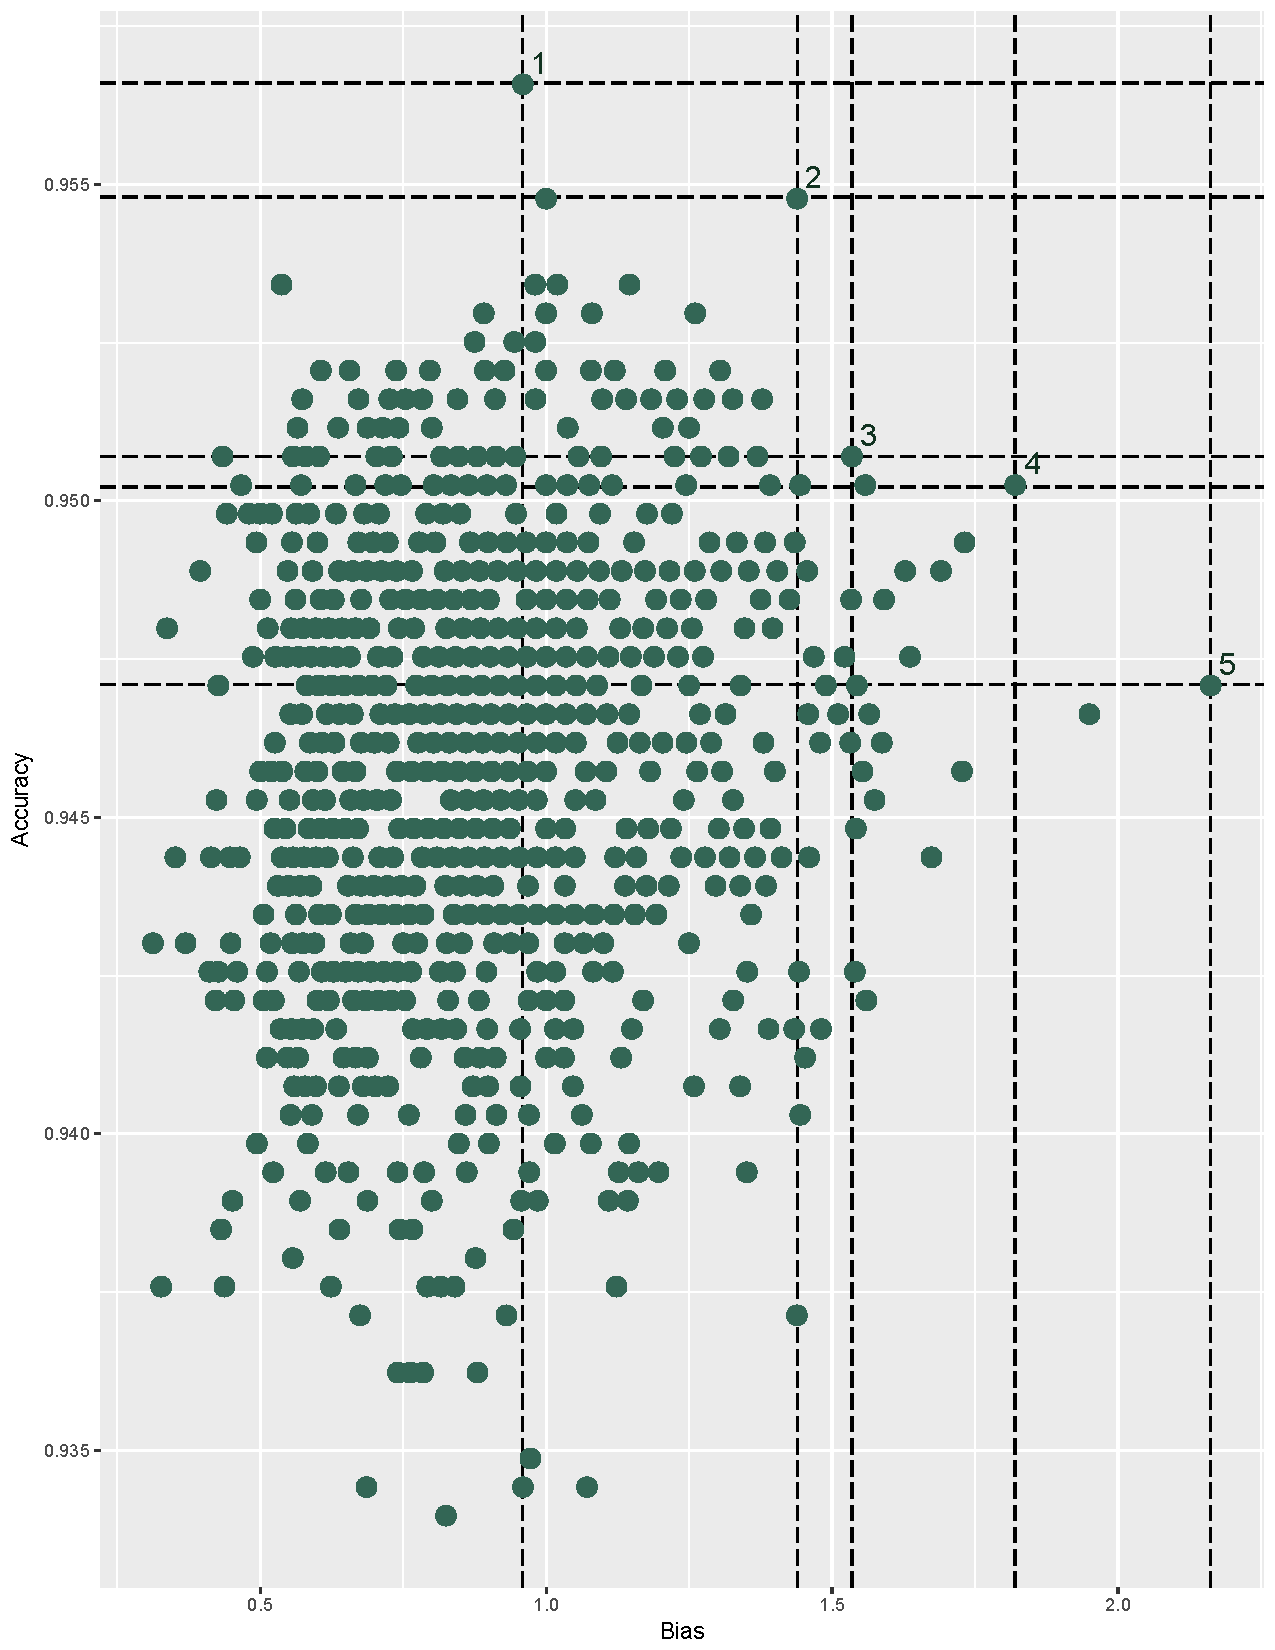
\includegraphics[width=0.65\linewidth]{Rplot04.pdf}}
{Bias - Accuracy Scatter Plot \label{fig1}}
{each dot represents one model with unique parameterization }
\end{figure}
%===============================



\section{Implications}

Machine learning hinges  on the quality of training data sets that feed into the underlying algorithm.  In ML,  the more objective the data and the larger the data set, the less possibility of distortion \citep{Rosso2015}.

\section {Concluding Remarks}

George Box, ``one of the great statistical minds of the 20th century'',  made the famous quote - ``all models are wrong, but some are useful'' \citep[p. 424]{box1987empirical}.  The aphorism today still shines a somewhat colder light on the much hyped and feared might of machine learning and AI. Decision analysis is  based on the maximum expected utility (MEU) action axiom, the basic proposition of which states that  human beings purposely utilize means in order to pursue  desired ends. To make high quality decisions, a decision-making agent (partnership between man and machine)  must have a sense of the association between various actions and the likelihood of different outcomes, as well as the desirability of each such outcome. Correspondingly, they represent prediction (from input features to output labels) and judgment (assign values to the expected utility of models derived). On the one hand,  latest advances in AI vastly  reduced the cost of prediction. On the other hand, AI also substantially raised the value of human judgment. To this end, we put forward our own version of Box's apothegm -    ``All models are biased, some are aggreably  preferreed''


%======================================================
% Acknowledgments here
\ACKNOWLEDGMENT{%
% Enter the text of acknowledgments here
}% Leave this (end of acknowledgment)


% Appendix here
% Options are (1) APPENDIX (with or without general title) or 
%             (2) APPENDICES (if it has more than one unrelated sections)
% Outcomment the appropriate case if necessary
%
% \begin{APPENDIX}{<Title of the Appendix>}
% \end{APPENDIX}
%
%   or 
%
% \begin{APPENDICES}
% \section{<Title of Section A>}
% \section{<Title of Section B>}
% etc
% \end{APPENDICES}
\newpage

%==========================================================
%\begin{table}
%\TABLE
%{The Villagers’ Benefit and Cost Matrix \label{tab1}}
%{\begin{tabular}{ccc}
%\hline 
%\up \down & \multicolumn{2}{c}{Perception }\\
%\hline 
%\up \down Reality & Wolf - Yes & Wolf - No\\
%\hline 
%\up Wolf & Respond and Rescue & Stay Put \\
 %\down -Yes& Time and Efforts well spent & Loss of Assets\\
%\hline 
%\up Wolf & Opportunity Cost & No Harm\\
%\down  -No& Waste of Time and Efforts & Zero Cost\\
%\hline
%\end{tabular}}
%{Adapted from \cite{doi:10.1175/1520-0434(2004)019<0391:TBWCWR>2.0.CO;2} }
%\end{table}
%================
%\begin{table}
%\TABLE
%{Sample Confusion Matrix \label{tab2}}
%{\begin{tabular}{ccc}
%\hline 
%\up \down & \multicolumn{2}{c}{Predicted Value}\\
%\hline 
%\up \down Actual & + & -\\
%\hline 
%\up + & True Positive (TP) & False Negative (FN) \\
% \down & Time and Efforts well spent & Loss of Assets\\
%\hline 
%\up - & False Positive (FP) & True Negative (TN)\\
%\down  & Waste of Time and Efforts & Zero Cost\\
%\hline
%\end{tabular}}
%{Adapted from \cite{7727750} }
%\end{table}
%==================================
%\begin{table}
%\TABLE
%{Performance Results \label{tab3}}
%{\begin{tabular}{clcc}
%\hline 
%\up \down Model &  Features &  Precision & Litmus Ratio \\
%\hline
%\up \down 1  &01 - 12  &  90\% & 0.78 \\
%\up \down 2 &  13 - 18 &  88\% & 0.24 \\
%\up \down 3  &  19 - 23 &  57\% & 0.01 \\
%\up \down 4  &  24 - 30 &  73\% & 0.57 \\
%\up \down 5  &  01 - 30  &  95\% & 1.27 \\
%\hline
%\end{tabular}}
%{Models differ in features included }
%\end{table}
%==================================
\newpage
%\begin{figure}
%\FIGURE
%{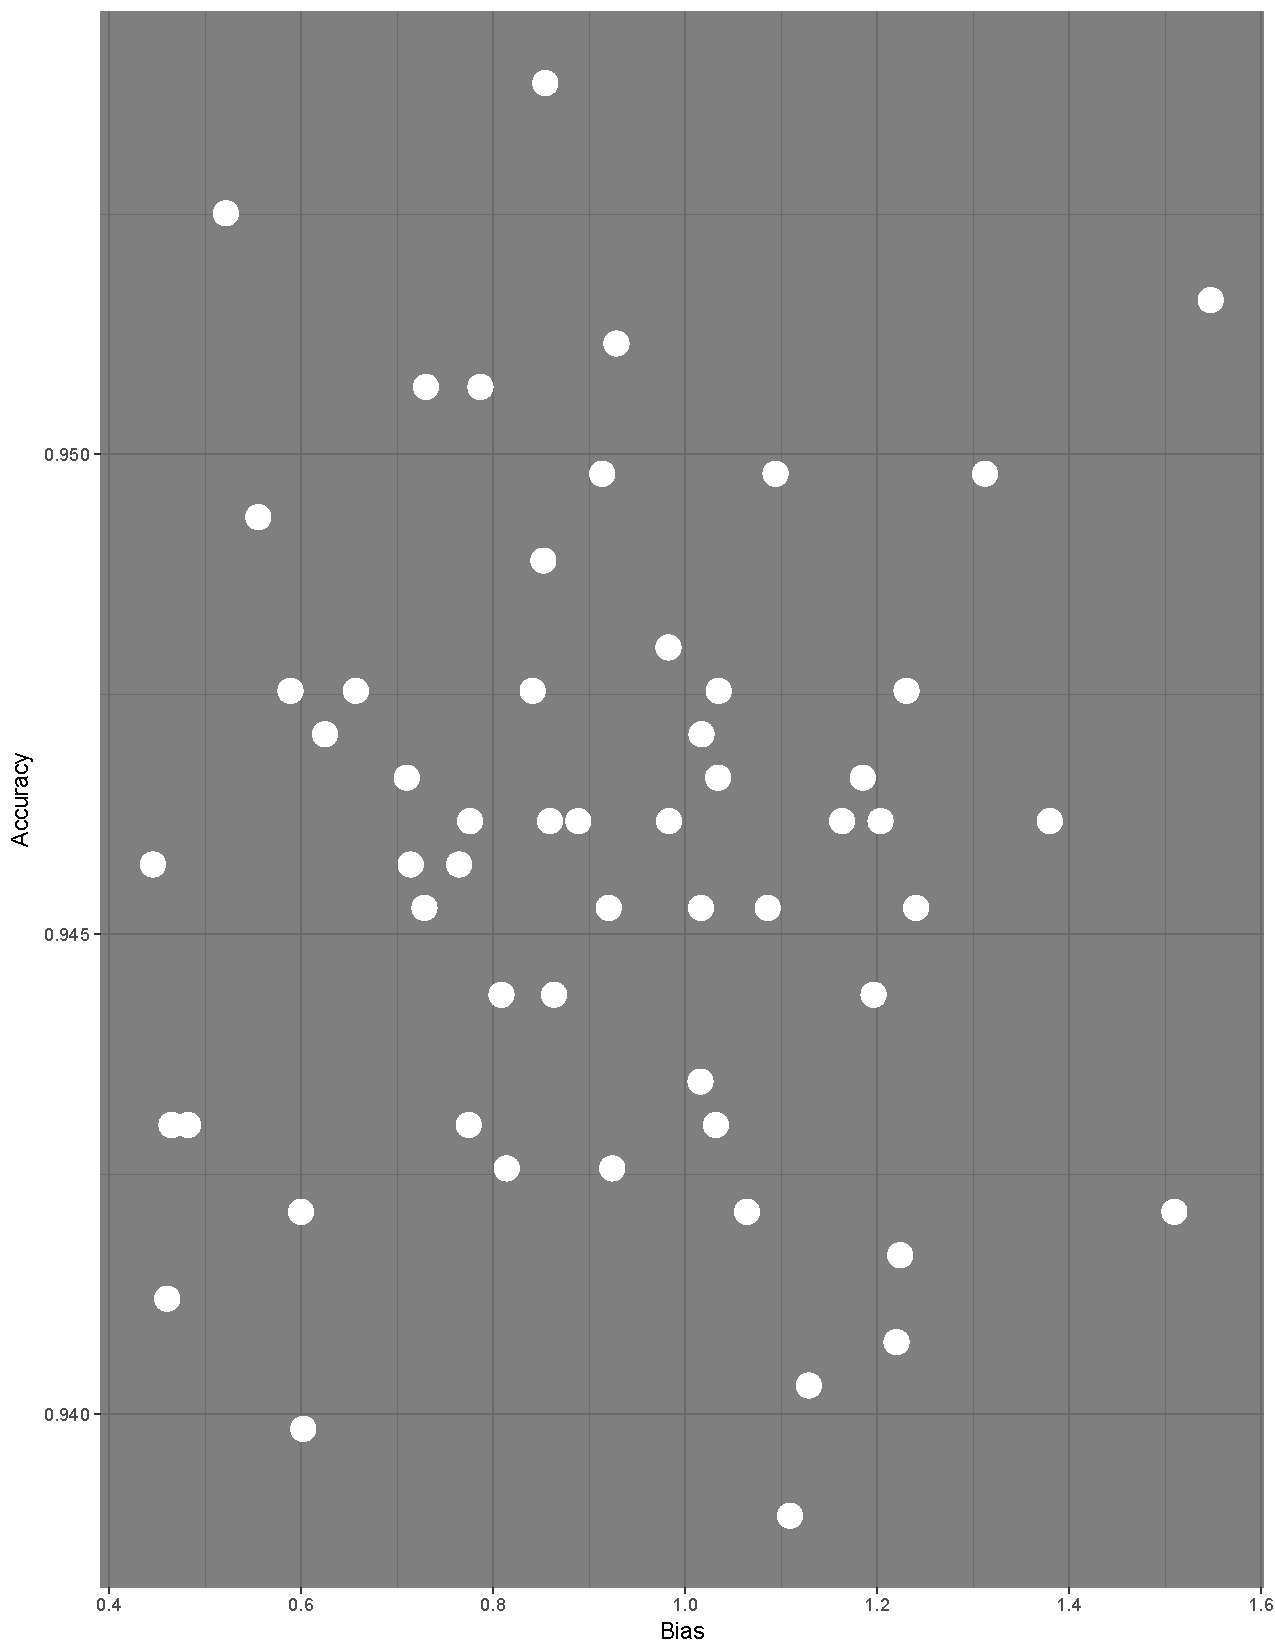
\includegraphics[width=0.5\linewidth]{Rplot.pdf}}
%{Figure Caption. \label{fig1}}
%{Text of Notes}
%\end{figure}


\newpage
% References here (outcomment the appropriate case) 

% CASE 1: BiBTeX used to constantly update the references 
%   (while the paper is being writduanten).
\bibliographystyle{informs2014} % outcomment this and next line in Case 1
\bibliography{duan} % if more than one, comma separated

% CASE 2: BiBTeX used to generate mypaper.bbl (to be further fine tuned)
%\input{mypaper.bbl} % outcomment this line in Case 2

\end{document}


